%TODO 制作导航部分
\begin{withoutheadline}
\begin{frame}
\vspace*{-13mm}
\begin{figure}
	\hspace*{-4.2mm}
    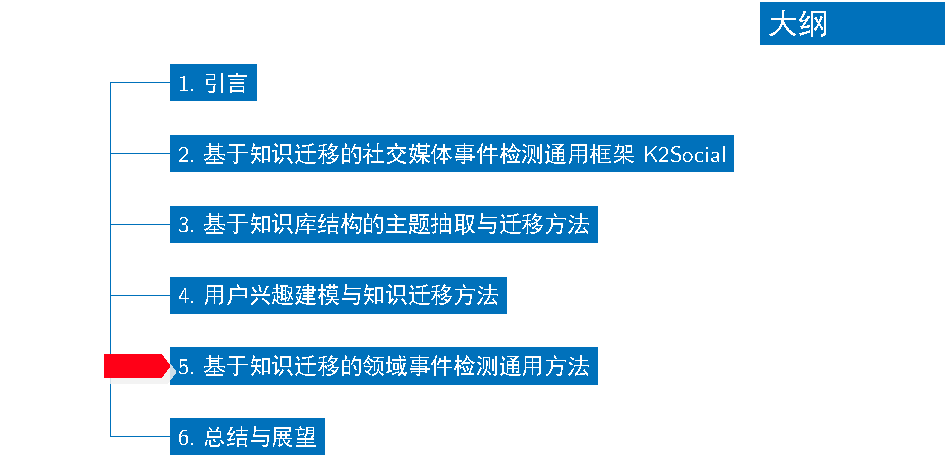
\includegraphics[width=1.0\paperwidth]{img/contents5_output.pdf}
\end{figure}

\end{frame}
\end{withoutheadline}

\section{基于知识迁移的领域事件检测通用方法}
%------------------------------
\begin{frame}
\frametitle{Motivation}
领域事件检测为什么是必须的?
\pdfnote{有什么合适的例子来说明领域事件检测呢?}
\end{frame}

%------------------------------
\begin{frame}
\frametitle{TaxoPhrase}	

\begin{figure}
	\caption{TaxoPhrase用于从维基百科知识库中抽取领域知识的示意图}
    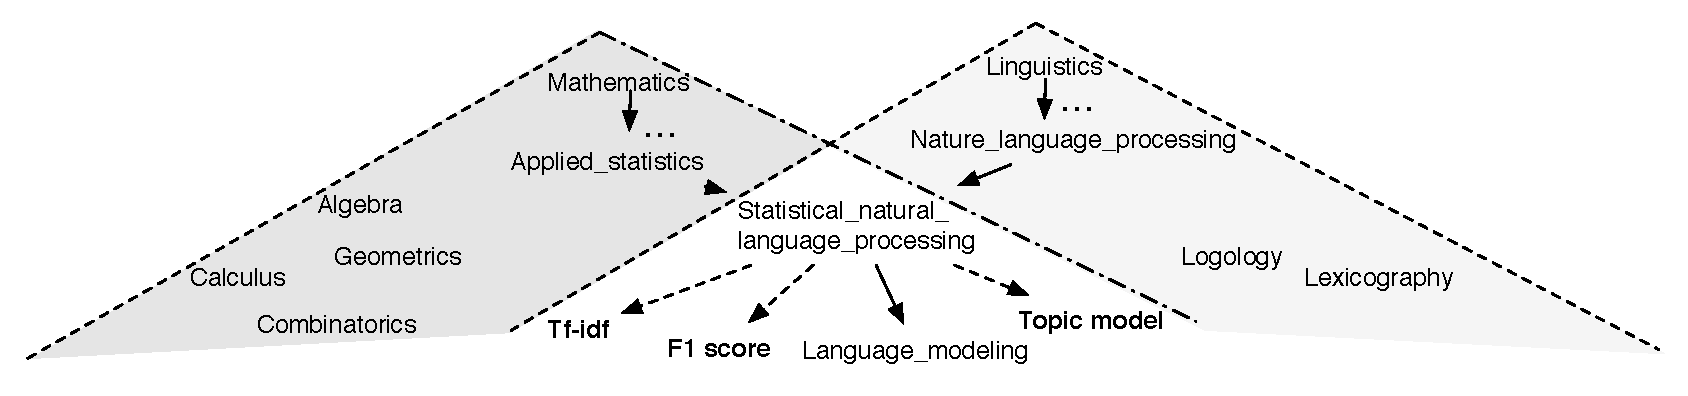
\includegraphics[width=1.0\textwidth]{img/TD+/taxophrase_motivation.pdf}
\end{figure}
\pdfnote{TaxoPhrase用于从知识库中抽取领域知识的示意图。用户1关心\textit{数学}领域中除\textit{统计自然语言处理}(白色区域)之外的知识(深灰色区域),用户2关心\textit{语言学}领域中除\textit{统计自然语言处理}之外的知识(浅灰色区域),在此场景中TaxoPhrase可将上述三部分用主题建模的方法加以探索与抽取。}
\end{frame}

%------------------------------
\begin{frame}
\frametitle{TaxoPhrase}	
\begin{figure}
	\caption{英文维基百科的分类体系中各类别节点的出度的分布}
    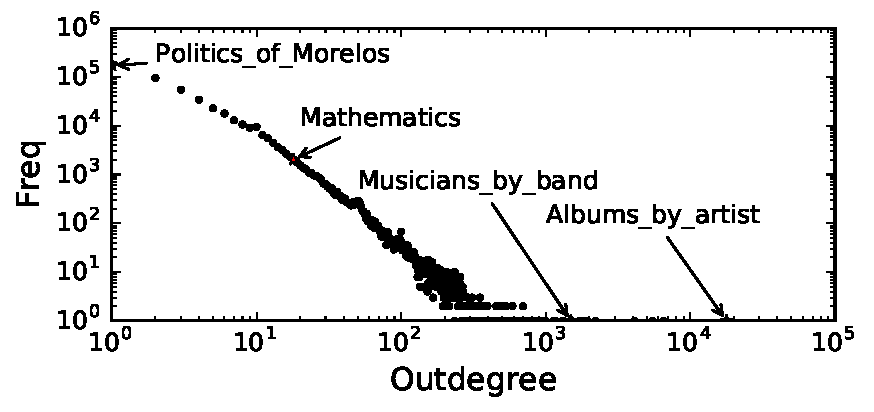
\includegraphics[width=1.0\textwidth]{img/TD+/outdegree_distribution.pdf}
\end{figure}
\end{frame}

%------------------------------
\begin{frame}
\frametitle{TaxoPhrase}	
\vspace{-5mm}
\begin{figure}
	\setlength{\abovecaptionskip}{0.cm}
	\setlength{\belowcaptionskip}{0.cm}
	\caption{知识库中有互补关系的三部分的示例}
    \includegraphics[width=0.75\textwidth]{img/TD+/example.pdf}
\end{figure}
\pdfnote{可以考虑给图的左侧加上分类类别、实体、短语的标注}
\end{frame}

%------------------------------
\begin{frame}
\frametitle{TaxoPhrase}
\begin{figure}
	\centering
	\caption{用于探索知识库中领域知识的概率模型TaxoPhrase的示意图}
    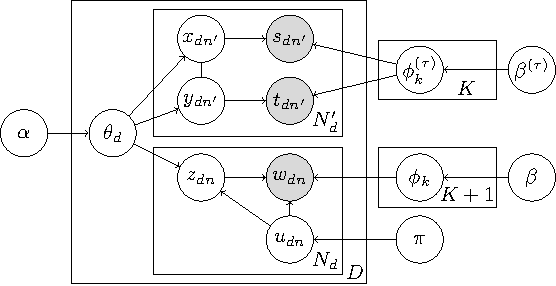
\includegraphics[width=0.8\columnwidth]{img/TD+/TaxoPhrase_inpaper.pdf}
	\label{fig:IllustrationTaxoPhrase}
\end{figure}
\end{frame}


%------------------------------
\begin{frame}
\frametitle{实验结果:TaxoPhrase的建模质量}	

\pdfnote{加TaxoPhrase在Maths上的建模结果}
\end{frame}


%------------------------------
\begin{frame}
\frametitle{实验结果:TaxoPhrase的建模质量}	

\begin{table}[]
\centering
\caption{各数据集统计信息,以及各方法获得的短语和分类类别两种主题的质量对比(以PMI为评测指标)}
\label{my-label}
\scalebox{0.8}{
\begin{tabular}{p{2.5cm}|l|r|r|r}
\hline
\multicolumn{2}{c|}{}           & Maths & Chemistry & Argentina \\
\hline
\multicolumn{2}{c|}{\#Entities} & 27,947 &  60,375 & 8,617 \\
%\hline
\multicolumn{2}{c|}{\#Category Types}  &     1,391        &3,038&	1,479\\
%\hline
\multicolumn{2}{c|}{\#Phrase Types}     &     116,013        &248,769&     21,183      \\
\hline
\hline
\multirow{2}{*}{on phrases} & LDA  &4.55 & 4.30 & 3.52 \\
&    TaxoPhrase &4.67& 4.55 & 3.81\\
\hline
\multirow{2}{*}{on categories} & SSN-LDA & 4.01 &3.97 &3.06\\
& TaxoPhrase & 4.51 &4.48& 3.73\\
\hline          
\end{tabular}
}
\label{tbl:taxophrase_dataset}
\end{table}
\end{frame}


%------------------------------
\begin{frame}
\frametitle{实验结果:TaxoPhrase抽取领域知识的实例}
\pdfnote{加TaxoPhrase在Feminism上的建模结果}
\end{frame}


%------------------------------
\begin{frame}
\frametitle{实验结果:TransDetector+领域事件检测}
\begin{table}
\centering
\setlength{\abovecaptionskip}{0.cm}
\setlength{\belowcaptionskip}{0.cm}
\caption{2011年6月30日至2011日9月15日,\textit{Edinburgh twitter corpus}数据集中Feminist(女权主义)相关事件列表及各事件检测方法在各事件上的具体表现}
\label{my-label}
\scalebox{0.65}{
\begin{threeparttable}  
\begin{tabular}{|c|l|c|c|c|c|c|c|c|}
\hline
\multirow{2}{*}{Date}  & \multirow{2}{*}{Representative event tweet} & \multirow{2}{*}{\begin{tabular}[c]{@{}l@{}}Number of \\ event tweet\end{tabular}} & \multicolumn{6}{c|}{Methods\tnote{a}} \\ \cline{4-9} 
 &  &  & L & TU & TW & E & B & TD+ \\ \hline
7/1/11  & \begin{tabular}[c]{@{}l@{}l@{}}DSK Has Bail Lifted Over \textbf{Sex Assault Case}:\\ Dominique Strauss-Kahn has had his bail\\ lifted after prosecutors said... http://bit.ly/llcWhN \end{tabular} & 46 & - & - & - & - & - & \checkmark \\ \hline
7/26/11 & \begin{tabular}[c]{@{}l@{}}bad! David Wu resigns because of an \textbf{unwanted}\\ \textbf{sexual encounter} with an 18-year-old \end{tabular} & 23 & - & - & - &  - & - & \checkmark  \\ \hline
8/17/11  & \begin{tabular}[c]{@{}l@{}l@{}} Nevin Shapiro said he provided players with \\ \textbf{sexual bribery} and cars over years, and\\ NCAA is investigating http://dlvr.it/cAaMF \end{tabular} & 52 & \checkmark & - & \checkmark & \checkmark & -  & \checkmark \\ \hline
8/19/11 & \begin{tabular}[c]{@{}l@{}l@{}l@{}l@{}} Obama relieves illegal immigrants who are\\ students, veterans, the elderly, crime victims\\ and those with family, including \textbf{same-sex partners} \end{tabular} & 21 & - & -  & \checkmark & - & -  & \checkmark \\ \hline
\end{tabular}

\begin{tablenotes}  
\item[a] L=LSH, TU=TimeUserLDA, TW, E=EDCoW, B=BurstyBTM, TD+=TaxoPhrase+\textsc{TransDetector}
\end{tablenotes}  
\end{threeparttable}  
}
\label{tbl:feminist_event_list}
\end{table}
\end{frame}


\begin{frame}
\frametitle{实验结果:TransDetector+领域事件检测}
\vspace{-7mm}
\begin{table}[!htbp]
\centering
\setlength{\abovecaptionskip}{2.mm}
\setlength{\belowcaptionskip}{1.mm}
\caption{\textit{Edinburgh twitter corpus}数据集中Natural Hazards(自然灾害)相关事件}
\label{my-label}
\scalebox{0.53}{
\begin{threeparttable}  
\begin{tabular}{|c|l|c|c|c|c|c|c|c|}
\hline
\multirow{2}{*}{Date}  & \multirow{2}{*}{Representative event tweet} & \multirow{2}{*}{\begin{tabular}[c]{@{}l@{}}Number of \\ event tweet\end{tabular}} & \multicolumn{6}{c|}{Methods\tnote{a}} \\ \cline{4-9} 
 &  &  & L & TU & TW & E & B & TD+ \\ \hline
7/2/11  & \begin{tabular}[c]{@{}l@{}l@{}}Exxon \textbf{oil spill} in Mont. river prompts\\ evacuations [AP] - An ExxonMobil pipeline that runs\\ under the Yellowstone River http://tiny.ly/IGuN \end{tabular} & 22 & - & - & - & - & - & \checkmark  \\ \hline
7/5/11 & \begin{tabular}[c]{@{}l@{}l@{}} @438PM Watching \textbf{storms} form around \#Phoenix,\\ potential for a \textbf{dust storm} 6-9PM. \#Tucson about\\ to get hit. \#azwx http://www.weather.gov/phoenix \end{tabular} & 40 & - & - & \checkmark &  - & - & \checkmark \\ \hline
7/11/11  & \begin{tabular}[c]{@{}l@{}l@{}} Possible \textbf{earthquake} east coast of\\ Honshu, JAPON ! 48hrs. close attention. \end{tabular} & 14 & - & - & - & - & - & \checkmark  \\ \hline
7/21/11  & \begin{tabular}[c]{@{}l@{}l@{}} DTN France: Deadly \textbf{heat-wave} spreads in US: A \\punishing \textbf{heat-wave} settles over the central and\\ eastern US, with ... http://bit.ly/q5mRkI. \end{tabular} & 249 & \checkmark & - & \checkmark & \checkmark & - & \checkmark  \\ \hline
8/23/11 & \begin{tabular}[c]{@{}l@{}l@{}l@{}l@{}} More
Virginia \textbf{Earthquake} 2011: Philadelphia\\ Eagles Feel Quake In Locker Room (VIDEO)\\ http://post.ly/2yOQ8 \end{tabular} & 310 & \checkmark & \checkmark  & \checkmark & \checkmark & \checkmark & \checkmark  \\ \hline
8/28/11 & \begin{tabular}[c]{@{}l@{}l@{}l@{}l@{}} @CBSBigBrother Anything but \textbf{Hurricane} \textbf{Irene} \end{tabular} & 1458 & \checkmark & \checkmark  & \checkmark & \checkmark & \checkmark & \checkmark  \\ \hline
9/1/11 & \begin{tabular}[c]{@{}l@{}l@{}l@{}l@{}} \textbf{Tropical storm} Lee in the Gulf of Mexico showed\\ up randomly like at mama's house looking to borrow \\a few dollars. \end{tabular} & 159 & \checkmark & -  & \checkmark & - & - & \checkmark  \\ \hline
9/5/11 & \begin{tabular}[c]{@{}l@{}l@{}l@{}l@{}} Satellite loop of the \textbf{wildfires} in Texas \\ http://fb.me/Zbve5o4E \end{tabular} & 21 & - & -  & - & \checkmark & - & \checkmark  \\ \hline
\end{tabular}

\begin{tablenotes}  
\item[a] L=LSH, TU=TimeUserLDA, TW, E=EDCoW, B=BurstyBTM, TD+=TaxoPhrase+\textsc{TransDetector}
\end{tablenotes}  
\end{threeparttable}  
}
\label{tbl:natural_hazards_event_list}
\end{table}
\end{frame}

\begin{frame}
\frametitle{TransDetector$^+$方法小结}

\begin{columns}
\column{0.75\textwidth}

\begin{enumerate}
	\item 提出了一种适用于各领域的领域事件检测通用方法TransDetector$^+$;
	\item 提出概率模型TaxoPhrase优化从知识库中抽取领域知识的过程;
	\item TransDetector$^+$将抽取出的领域知识迁移至社交媒体数据流中,检测领域事件;
	\item 在4个示例领域中进行实验,相较于已有方法,平均将F值提升了21\%
\end{enumerate}

\column{0.25\textwidth}

\end{columns}

\pdfnote{本文提出了一种适用于各领域的领域事件检测通用方法TransDetector+。TransDetector+方法利用本文提出的概率模型TaxoPhrase优化从知识库中抽取领域知识的过程,并将抽取出的领域知识迁移至社交媒体数据流中,提取和领域相关的词和短语的时间序列,进而检测领域事件。TransDetector+在4个示例领域中进行了实验,相较于已有方法,平均将F值提升了21\%}

\end{frame}
